\pgfplotscreateplotcyclelist{custom list}{%
Dark2-8-1,
Dark2-8-2,
Dark2-8-3,
Dark2-8-4,
Dark2-8-5,
Dark2-8-6,
Dark2-8-7,
Dark2-8-8,
Set1-9-1,
Set1-9-2,
Set1-9-3,
Set1-9-4,
Set1-9-5,
Set1-9-6,
Set1-9-7,
Set1-9-8,
Set1-9-9}

With the knowledge of \glspl{crn} and \gls{ga}, we now move on to discuss the two models of delay line implemented as a \gls{crn}. First, a model of the delay line that has greater precision, but requires more control signals. Then, the second model requires fewer control signals, but it comes at the cost of precision. Both models are then connected with a \gls{asp} to demonstrate functionality and modularity. This chapter is based off our accepted paper~\cite{Moles2014-ia}.

\section{Delay Line Concept}

A delay line is a way to store data in an ordered fashion over time. The delay line we design operates similar to a \gls{fifo} data buffer, but allows random access to any element of the \gls{fifo}. Figure~\ref{fig:delay_line_general} shows an example of a delay line shifting values down. Table~\ref{tab:delay_line_general} shows an example of how values shift down with increasing time, $t$.

\begin{figure}
    \centering
    \begin{tikzpicture}
        [c1/.style={circle,draw=black!50,fill=Accent-4-1,thick},
         b1/.style={rectangle,draw=black!50,fill=Accent-4-2,thick},
         b2/.style={rectangle,draw=white!50,fill=white!50,thick}]
        \node[c1]    (cirt0)        {x};
        \node[b1]    (boxt0)        [right=of cirt0]        {$x(t)$}
            edge[<-]    (cirt0);
        \node[b1]    (boxt1)        [right=0.2cm of boxt0]    {$x(t-1)$}
            edge[<-]    (boxt0);
        \node[b1]    (boxt2)        [right=0.2cm of boxt1]    {$x(t-2)$}
            edge[<-]    (boxt1);
        \node[b2]    (boxte)        [right=0.2cm of boxt2]    {\ldots}
            edge[<-]    (boxt2);
        \node[b1]    (boxtn)        [right=0.2cm of boxte]    {$x(t-n)$}
            edge[<-]    (boxte);
    \end{tikzpicture}
    \caption[Delay Line]{Diagram of an example delay line. The circle, $x$, is the input value and box $x(t)$ represents the value of $x$ at current time step. Box labeled $x(t-1)$ represents one time step ago, $x(t-2)$ represents two time steps ago, and so on.}
    \label{fig:delay_line_general}
\end{figure}
    
\begin{table}
    \centering
    \begin{tabular}{l|l|l l l l}
    \textbf{t} & $\mathbf{x}$ & $\mathbf{x(t)}$ & $\mathbf{x(t-1)}$ & $\mathbf{x(t-2)}$ & $\mathbf{x(t-3)}$ \\ \hline
    0 & 15 & 15 & ~  & ~  & ~  \\
    1 & 19 & 19 & 15 & ~  & ~  \\
    2 & 12 & 12 & 19 & 15 & ~  \\
    3 & 14 & 14 & 12 & 19 & 15 \\
    4 & 11 & 11 & 14 & 12 & 19 \\
    \end{tabular}
    \caption[Delay Line Values Over Time]{Table of values for a given input value, $x$, and how they shift through a delay line. Each value, $t-n$, represents the value $n$ time steps ago.}
    \label{tab:delay_line_general}
\end{table}

\section{Delay Line Design}
\label{sec:delayline}
To introduce the time delay line design, we will first examine a delay line constructed of only two stages in two different styles. One is a \acrfull{mdl} that requires experimenter participation to indicate when it is time to move values between stages. The second model automatically propagates the signaling species backwards, hence it is more autonomous, but it comes at the cost of additional and cumulative error in the resulting output values.

\subsection{Manual Copy Delay Line}
First, we will introduce the delay line of two stages with manual copy of the signaling species shown in Figure~\ref{fig:manualprop_n_2}. A delay line of two stages is composed of seven species: $X$, $X1C$, $X1$, $X2$, $X2C$, $X2_{signal}$, and $X1_{signal}$. The species $X$ represents the input value of the delay line. The signaling species, $X1_{signal}$ and $X2_{signal}$, are the catalysts that start the reaction conversion of $X$ into corresponding stages. The primary function of $X1_{signal}$ is to trigger and accelerate the copy reaction which converts of $X$ to $X1C$ and $X1$. Species $X2_{signal}$ performs a similar action for the conversion of $X1C$ to $X2$.

Species $X1C$ and $X2C$ are delayed copies of $X$ that move to the next stage of the system (for example, $X1$ to $X2$ and $X2C$). Species $X2C$ is shown for completeness and is used to cascade the system to a delay line of more than two stages. For a two stage delay line, $X2C$ is waste and flushed. The outputs of the system are the $X1$ and $X2$ species, i.e., $X1$ and $X2$ represent the current and previous values of $X$ that are consumed as the inputs of another system.

\newsavebox\syringebox
\begin{lrbox}{\syringebox}
    \begin{tikzpicture}[y=0.80pt, x=0.8pt,yscale=-1, inner sep=0pt, outer sep=0pt]
  \path[draw=black,fill=cc0c0c0,line join=round,line cap=round,miter
    limit=4.00,even odd rule,line width=6.400pt] (104.8628,4.3331) --
    (100.3003,8.8018) -- (105.9566,14.5831) -- (93.3003,27.0206) --
    (101.6128,35.5206) -- (114.3003,23.0831) -- (119.9566,28.8643) --
    (124.5191,24.3956) -- (104.8628,4.3331) -- cycle(88.6441,22.5518) --
    (41.6128,68.6143) -- (58.9566,86.3331) -- (105.9566,40.2393) --
    (88.6441,22.5518) -- cycle(47.7378,74.9581) -- (37.3941,85.0831) --
    (38.7066,86.4268) -- (6.5816,116.6768) -- (4.9878,122.6456) --
    (40.8316,88.5831) -- (42.5503,90.3331) -- (52.8941,80.2393) --
    (47.7378,74.9581) -- cycle;
\begin{scope}[shift={(183.219,-198.691)}]
  \path[shift={(-183.219,198.691)},fill=cc0c0c0,line join=miter,line
    cap=butt,miter limit=4.00,even odd rule,line width=2.400pt] (39.3665,85.8168)
    -- (6.5814,116.6794) -- (4.9851,122.6552) -- (41.4219,87.9924) --
    (39.3665,85.8168) -- cycle;
  \path[cm={{0.69985,0.71429,-0.71429,0.69985,(-183.219,198.691)}},draw=black,fill=cffffff,line
    join=round,line cap=round,miter limit=4.00,nonzero rule,line
    width=1.805pt,rounded corners=0.0000cm] (78.1378,-47.5230) rectangle
    (102.9168,18.3064);
  \path[cm={{0.69985,0.71429,-0.71429,0.69985,(-183.219,198.691)}},draw=black,fill=cffffff,line
    join=round,line cap=round,miter limit=4.00,nonzero rule,line
    width=1.805pt,rounded corners=0.0000cm] (84.5786,-71.0885) rectangle
    (96.4759,-47.7304);
  \path[cm={{0.69985,0.71429,-0.71429,0.69985,(-183.219,198.691)}},draw=black,fill=cffffff,line
    join=round,line cap=round,miter limit=4.00,nonzero rule,line
    width=1.805pt,rounded corners=0.0000cm] (76.4862,-71.8876) rectangle
    (104.5683,-65.4768);
  \path[cm={{0.69985,0.71429,-0.71429,0.69985,(-183.219,198.691)}},draw=black,fill=cb3b3b3,line
    join=round,line cap=round,miter limit=4.00,nonzero rule,line
    width=1.805pt,rounded corners=0.0000cm] (86.9479,18.3706) rectangle
    (94.3150,32.8346);
  \path[fill=cb3b3b3,line join=round,line cap=round,miter limit=4.00,nonzero
    rule,line width=1.645pt] (-128.3155,255.9149) -- (-96.0548,255.7926) --
    (-124.1199,283.6438) -- (-140.4350,267.5587) -- (-128.3155,255.9149) -- cycle;
  \path[shift={(-183.219,198.691)},draw=black,fill=c00ffff,line join=round,line
    cap=round,miter limit=4.00,even odd rule,line width=1.805pt] (65.9531,78.7460)
    .. controls (57.7865,70.4108) and (57.9323,70.5597) .. (57.9323,70.5597);
  \path[shift={(-183.219,198.691)},draw=black,fill=c00ffff,line join=round,line
    cap=round,miter limit=4.00,even odd rule,line width=1.805pt] (74.5488,70.3242)
    .. controls (66.3821,61.9890) and (66.5280,62.1378) .. (66.5280,62.1378);
  \path[shift={(-183.219,198.691)},draw=black,fill=c00ffff,line join=round,line
    cap=round,miter limit=4.00,even odd rule,line width=1.805pt] (83.1444,61.9023)
    .. controls (74.9777,53.5671) and (75.1236,53.7160) .. (75.1236,53.7160);
  \path[shift={(-183.219,198.691)},draw=black,fill=c00ffff,line join=round,line
    cap=round,miter limit=4.00,even odd rule,line width=1.805pt] (91.7400,53.4804)
    .. controls (83.5734,45.1453) and (83.7192,45.2941) .. (83.7192,45.2941);
\end{scope}

\end{tikzpicture}


\end{lrbox}

\newcommand \syringePDFImage{\usebox\syringebox}

\begin{figure}[ht]
	\centering
	\begin{tikzpicture}
		[t1/.style={circle,draw=black!100,fill=Accent-4-1,thick},
		 tsig/.style={circle,draw=black!100,fill=Accent-4-1,thick},
		 t2/.style={circle,draw=black!100,fill=Accent-4-2,thick},
		 t3/.style={circle,draw=black!100,fill=Accent-4-3},
		 lmb/.style={circle,draw=white!100,fill=white!50}]

		\node[t1]	(xinj)		{$X$};
		\node[t2]	(x1)		[below right=of xinj]	{$X1$};
		\node[t3]	(x1c)		[below left=of xinj]	{$X1C$};
		\node[t2]	(x2)		[below right=of x1c]	{$X2$};
		\node[t3]	(x2c)		[below left=of x1c]		{$X2C$};
		\node[tsig]	(x2sig)		[left=of x1c]			{$X2_{signal}$};
		\node[tsig] (x1sig)     [left=of xinj]			{$X1_{signal}$};
		\node[lmb]  (lamb)		[above=of x1sig]		{$\lambda$};
		\node[lmb]  (lamb2)		[above=of x2sig]		{$\lambda$};

		\node[scale=0.2]	(syr1)		[above right=-0.1cm of xinj]	{\syringePDFImage};
		\node[scale=0.2,rotate=90]	(syr2)		[above left=0.1cm of x2sig]	{\syringePDFImage};
		\node[scale=0.2,rotate=90]	(syr3)		[above left=0.1cm of x1sig]	{\syringePDFImage};

		\draw[->,thick] (xinj.south) -- ($(x1c.north)!0.5!(x1.north)$) to[out=-90,in=0] (x1c.east);
		\draw[->,thick] (xinj.south) -- ($(x1c.north)!0.5!(x1.north)$) to[out=-90,in=180] (x1.west);

		\draw[->,thick] (x1c.south) -- ($(x2c.north)!0.5!(x2.north)$) to[out=-90,in=0] (x2c.east);
		\draw[->,thick] (x1c.south) -- ($(x2c.north)!0.5!(x2.north)$) to[out=-90,in=180] (x2.west);

		\draw[->,dashed,thick] (x1sig.south east) -- ($(x1c.north)!0.5!(x1.north)$);
		\draw[->,dashed,thick] (x2sig.south east) -- ($(x2c.north)!0.5!(x2.north)$);

		\draw[->,thick] (x2sig.north) to[out=90,in=270] (lamb2.south);
		\draw[->,thick] (x1sig.north) to[out=90,in=270] (lamb.south);

	\end{tikzpicture}
	\caption[Two Stage Manual Copy Delay Line]{\Gls{mdl} with two stages. The syringe is used to indicate the species where inputs are presented and $X1$ and $X2$ represent the output species from the delay line. Species $X2C$ is used to cascade a value to a delay line of greater than two stages. The signal species, $X1_{signal}$ and $X2_{signal}$, catalyze the copy reactions and are removed from the system by decay ($\lambda$).}
	\label{fig:manualprop_n_2}
\end{figure}

Species $X1C$ is the internal transition storage species. The storage species acts as a buffer for the value that will transition into $X2$ on next activation of the system with an $X2_{signal}$ passed in. Ideally, the concentration of $X1C$ will be the same as $X1$ prior to its consumption. This process is represented by a set of reactions using the previously mentioned species. Reactions~\ref{eq:XreacMan}~and~\ref{eq:X1CreacMan} (below) represent the conversion of the input species, $X$, through to the output species, $X1$ and $X2$.
\begin{alignat}{2}
X & \xrightarrow{X1_{signal}} & X1 + X1C  \label{eq:XreacMan} \\
X1C & \xrightarrow{X2_{signal}} & X2 + X2C \label{eq:X1CreacMan}
\end{alignat}
Reactions~\ref{eq:X2sigMan} and \ref{eq:X1sigMan} show the decay (represented by lambda, $\lambda$) of the catalyst species, $X1_{signal}$ and $X2_{signal}$.
\begin{alignat}{2}
X2_{signal} & \rightarrow & \lambda \label{eq:X2sigMan} \\
X1_{signal} & \rightarrow & \lambda \label{eq:X1sigMan}
\end{alignat}

Now, using these reactions, we can examine data moving through the delay line. For this \gls{mdl}, actions must occur at two moments (in time). First, at time zero, we present a random value to the input $X$ and reset $X1$ and $X2$ to zero. The reset of $X1$ and $X2$ simulate consumption by the underlying system the delay line is integrated with. Species $X2_{signal}$ is set to one to copy the value stored in $X1C$ to $X2$. In the ideal case for the initialization and first run of the delay line, $X2$ should be zero until these actions repeat. After 25 time steps, $X1_{signal}$ is injected to the system. The wait is to fully allow the transition of $X1C$ to $X2$ before beginning the transformation of $X$ to $X1C$. These injections repeat every 1,000 time steps and are summarized in Table~\ref{tab:as2Man}. Table~\ref{tab:as2Pipeline} shows an example of these injections repeating every 1,000 time steps with example data moving through.

\begin{table}[ht]
	\caption[Two Stage Manual Delay Line Actions]{Actions for two stage \gls{mdl} simulations.}
	\label{tab:as2Man}
	\centering
	\begin{tabular}{lll}
		Time		& Species			& Value 					\\ \hline
		0			& $X$				& $0.0 \le rand() \le 1.0$	\\
		0			& $X1$				& 0							\\
		0			& $X2$				& 0							\\
		0			& $X2_{Signal}$ 	& 1							\\
		25			& $X1_{Signal}$ 	& 1							\\
	\end{tabular}
\end{table}

\begin{table}
	\centering
	\caption[Pipeline View of Data in Two Stage Manual Delay Line]{Pipeline view of data moving through manual signaling delay line from Table~\ref{tab:as2Man}. Bold items show those injected to the system. \textbf{A}, \textbf{B}, and \textbf{C} are inputs and \textbf{1} is a concentration (presence) of $Xm_{signal}$.}
	\label{tab:as2Pipeline}
    \begin{tabular}{l|l|l|l|l|l|l}
    Species  & Time=0                     & 25                         & 1000                       & 1025                       & 2000                       & 2025                       \\ \hline
    X        & $\textbf{A}$               & $A \rightarrow 0$          & $\textbf{B}$               & $B \rightarrow 0$          & $\textbf{C}$               & $C \rightarrow 0$          \\
    X1signal & ~                          & $\textbf{1} \rightarrow 0$ & ~                          & $\textbf{1} \rightarrow 0$ & ~                          & $\textbf{1} \rightarrow 0$ \\
    X2signal & $\textbf{1} \rightarrow 0$ & ~                          & $\textbf{1} \rightarrow 0$ & ~                          & $\textbf{1} \rightarrow 0$ & ~                          \\ \hline
    X1       & $\textbf{0}$               & $0 \rightarrow A$          & $\textbf{0}$               & $0 \rightarrow B$          & $\textbf{0}$               & $0 \rightarrow C$          \\
    X1C      & ~                          & $\rightarrow A$            & $A \rightarrow 0$          & $0 \rightarrow B$          & $B \rightarrow 0$          & $0 \rightarrow C$          \\
    X2       & $\textbf{0}$               & ~                          & $\textbf{0} \rightarrow A$ & $A$                        & $\textbf{0} \rightarrow B$ & $B$                        \\
    X2C      & ~                          & ~                          & $\rightarrow A$            & $A$                        & $A \rightarrow B$          & $B$                        \\
    \end{tabular}
\end{table}

Figures~\ref{fig:delay2allMan_A} and ~\ref{fig:delay2allMan_B} shows the results of running the actions in Table~\ref{tab:as2Man} for 10 iterations (10,000 time steps). Valid data is available for examination on output species $X1$ and $X2$ every time steps after each cycle. Figure~\ref{fig:delay2XMan} shows the input values injected to the manual delay line. During the first cycle, species $X2$ remains at zero since there is no previous value as seen in Figure~\ref{fig:delay2X1Man}. Figure~\ref{fig:delay2X2SignalMan} shows the catalysts, $X2_{signal}$ and $X1_{signal}$, sequentially injected each cycle. Figure~\ref{fig:delay2X2SignalZoomedMan} presents the sequence of actions where $X2_{signal}$ is injected at time zero followed by $X1_{signal}$ 25 time steps later.

\begin{figure}[ht]
	\centering
	\begin{subfigure}[b]{0.9\textwidth}
	    \centering
		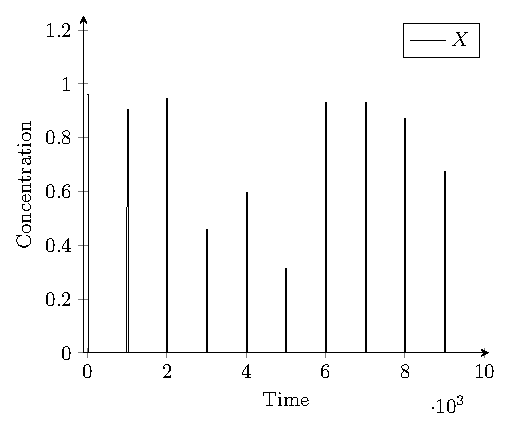
\includegraphics[width=9cm]{ac_3505_as_1979_t_10000_x1Inj}
		\caption{Input}
		\label{fig:delay2XMan}
		\vspace{15mm}
	\end{subfigure}
	\\
	\begin{subfigure}[b]{0.9\textwidth}
	    \centering
		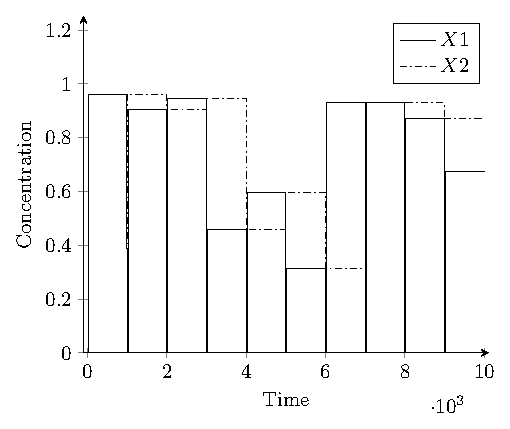
\includegraphics[width=9cm]{ac_3505_as_1979_t_10000_x1_x2}
		\caption{Outputs}
		\label{fig:delay2X1Man}
	\end{subfigure}
	\caption[Two Stage Manual Copy Delay Line I/O]{Two stage \gls{mdl} showing input and output signals. Data arrives as input (\ref{fig:delay2XMan}) and is available on outputs (\ref{fig:delay2X1Man}) with $X1$ being the current and $X2$ being the previous $X$.}
	\label{fig:delay2allMan_A}
\end{figure}

\begin{figure}[ht]
    \centering
	\begin{subfigure}[b]{0.9\textwidth}
	    \centering
		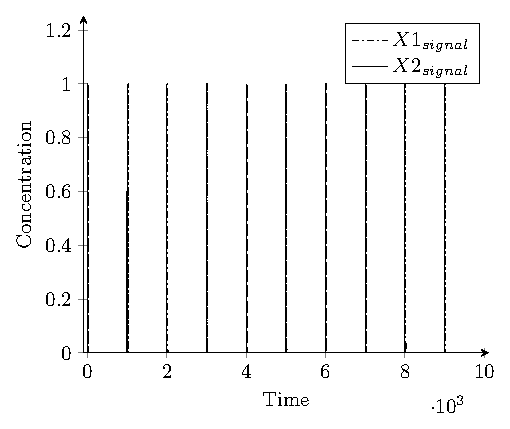
\includegraphics[width=9cm]{ac_3505_as_1979_t_10000_x1signal_x2signal}
		\caption{Copy Signals}
		\label{fig:delay2X2SignalMan}
		\vspace{15mm}
	\end{subfigure}
	\\
	\begin{subfigure}[b]{0.9\textwidth}
	    \centering
		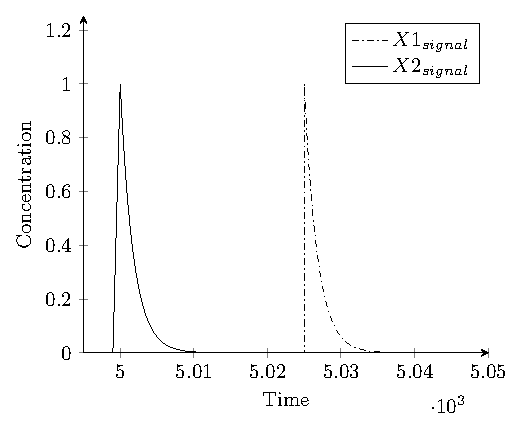
\includegraphics[width=9cm]{ac_3505_as_1979_t_10000_x1signal_x2signal_zoomed}
		\caption{Copy Signals (Zoomed on Figure~\ref{fig:delay2X2SignalMan})}
		\label{fig:delay2X2SignalZoomedMan}
	\end{subfigure}
	\caption[Two Stage Manual Copy Delay Line Signaling]{Two stage \gls{mdl} showing the copy signals. The copy of this data is triggered by $X1_{signal}$ and $X2_{signal}$ (\ref{fig:delay2X2SignalMan}). Figure~\ref{fig:delay2X2SignalZoomedMan} shows the copy signals zoomed in from Figure~\ref{fig:delay2X2SignalMan}.}
	\label{fig:delay2allMan_B}
\end{figure}

\subsection{Backwards Signal Propagation Delay Line}
The \acrfull{bpl} handles the signal species differently. More specifically, the only input signaling species is $X2_{signal}$ and rather than decay, $X2_{signal}$ reacts to $X1_{signal}$. The advantage of this model is that the user is only required to perform actions at the beginning of the cycle and then the system transforms the species internally (without external help). Figure~\ref{fig:delayelement} shows a revision of the \gls{mdl} for this model. This reduces the number of injections to two: the input ($X$) and the final copy signal ($X2_{signal}$ for two stage). The change leaves reactions~\ref{eq:Xreac} and \ref{eq:X1Creac} unchanged.

\begin{figure}[ht]
	\centering
	\begin{tikzpicture}
		[t1/.style={circle,draw=black!100,fill=Accent-4-1,thick},
		 tsig/.style={circle,draw=black!100,fill=Accent-4-1,thick},
		 t2/.style={circle,draw=black!100,fill=Accent-4-2,thick},
		 t3/.style={circle,draw=black!100,fill=Accent-4-3},
		 lmb/.style={circle,draw=white!100,fill=white!50}]

		\node[t1]	(xinj)		{$X$};
		\node[t2]	(x1)		[below right=of xinj]	{$X1$};
		\node[t3]	(x1c)		[below left=of xinj]	{$X1C$};
		\node[t2]	(x2)		[below right=of x1c]	{$X2$};
		\node[t3]	(x2c)		[below left=of x1c]		{$X2C$};
		\node[tsig]	(x2sig)		[left=of x1c]			{$X2_{signal}$};
		\node[tsig] (x1sig)     [left=of xinj]			{$X1_{signal}$};
		\node[lmb]  (lamb)		[above=of x1sig]		{$\lambda$};			

		\node[scale=0.2]	(syr1)		[above right=-0.1cm of xinj]	{\syringePDFImage};
		\node[scale=0.2,rotate=90]	(syr2)		[above left=0.1cm of x2sig]	{\syringePDFImage};

		\draw[->,thick] (xinj.south) -- ($(x1c.north)!0.5!(x1.north)$) to[out=-90,in=0] (x1c.east);
		\draw[->,thick] (xinj.south) -- ($(x1c.north)!0.5!(x1.north)$) to[out=-90,in=180] (x1.west);

		\draw[->,thick] (x1c.south) -- ($(x2c.north)!0.5!(x2.north)$) to[out=-90,in=0] (x2c.east);
		\draw[->,thick] (x1c.south) -- ($(x2c.north)!0.5!(x2.north)$) to[out=-90,in=180] (x2.west);

		\draw[->,dashed,thick] (x1sig.south east) -- ($(x1c.north)!0.5!(x1.north)$);
		\draw[->,dashed,thick] (x2sig.south east) -- ($(x2c.north)!0.5!(x2.north)$);

		\draw[->,thick] (x2sig.north) to[out=90,in=180] (x1sig.west);
		\draw[->,thick] (x1sig.north) to[out=90,in=270] (lamb.south);

	\end{tikzpicture}
	\caption[Two Stage Backwards Propagating Delay Line]{Backwards propagating delay design with two stages. The syringe is used to indicate an injection of the input species $X$ and the copy signal $X2_{signal}$. The species $X1$ and $X1$ represent the output species from the delay line. The signal $X2_{signal}$ is propagated backwards to $X1_{signal}$ without user intervention and then decays ($\lambda$).}
	\label{fig:delayelement}
\end{figure}

\begin{alignat}{2}
X & \xrightarrow{X1_{signal}} & X1 + X1C  \label{eq:Xreac} \\
X1C & \xrightarrow{X2_{signal}} & X2 + X2C\label{eq:X1Creac}
\end{alignat}

Revising the remaining reactions requires modifying only reaction~\ref{eq:X2sigMan}. Removing the decay from reaction~\ref{eq:X2sigMan} so that $X2_{signal}$ reacts to $X1_{signal}$ gives the updated reactions~\ref{eq:X2sig} and \ref{eq:X1sig}.

\begin{alignat}{2}
X2_{signal} & \rightarrow & X1_{signal} \label{eq:X2sig} \\
X1_{signal} & \rightarrow & \lambda \label{eq:X1sig}
\end{alignat}

All actions in the system occur instantaneously and are the same as actions employed by the manual delay line at time zero. At the beginning of every cycle, $X1$ and $X2$ are set to zero to simulate the next block of the system consuming their values. Also, a random value ($X$) and signal ($X2_{signal}$) are injected to the system. Table~\ref{tab:as2} summarizes these actions, which repeat every 1,000 time steps to ensure enough time for all reactions to reach steady state.

\begin{table}
	\caption[Two Stage Backwards Propagation Delay Line]{Actions for two stage back propagation delay line simulations. These actions repeat every 1000 similar to Table~\ref{tab:as2Pipeline}.}
	\label{tab:as2}
	\centering
	\begin{tabular}{lll}
		Time		& Species			& Value 					\\ \hline
		0			& $X$				& $0.0 \le rand() \le 1.0$	\\
		0			& $X1$				& 0							\\
		0			& $X2$				& 0							\\
		0			& $X2_{Signal}$ 	& 1							\\
	\end{tabular}
\end{table}

The simulations of the \gls{bpl} run for 10,000 time steps (same as for the manual delay line). Valid data is also produced at the same point (every 50 steps) on the output species $X1$ and $X2$. The value produced on the first cycle of $X2$ ideally should be zero, but leakage from $X1C$ is generally seen from steps zero to 1,000 (see Figure~\ref{fig:delay2X1}). An input is introduced to the system at species $X$ (Figure~\ref{fig:delay2X}) and then is reacted in the same cycle to species $X1$ (Figure~\ref{fig:delay2X1}). After the next cycle (i.e., the next introduction of $X2_{signal}$), the value injected at $X$ previously is now presented at $X2$ (Figure~\ref{fig:delay2X1}).

Notice that the backwards propagation introduces an error to the system with some of the $X2$ values not lining up exactly with the previous $X1$. This difference is due to the time window that the reactions for $X$ to $X1$ and $X1$ to $X2$ are simultaneously active. Looking at Figure~\ref{fig:delay2X2SignalZoomed}, $X1_{signal}$ and $X2_{signal}$ are large enough for both catalyses to occur. So, for this small window of time, there is effectively a direct path from $X$ to cascade down to $X2$. This overlap is not inherently a problem. It allows the desired parallelism of this system. We can afford this error in a small number of stages, but the inaccuracy can grow with a larger number of stages.

\begin{figure}[ht]
	\centering
	\begin{subfigure}[b]{0.9\textwidth}
	    \centering
		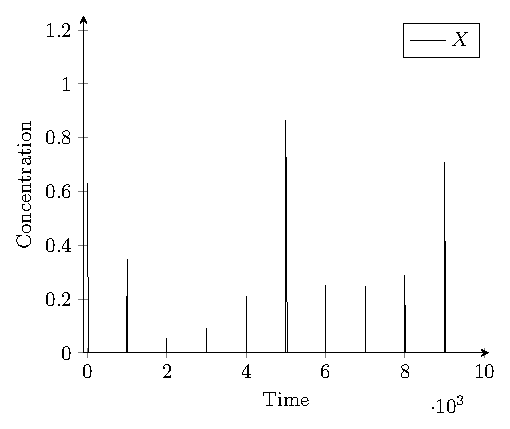
\includegraphics[width=9cm]{ac_3502_as_1957_t_10000_x1Inj}
		\caption{Input}
		\label{fig:delay2X}
		\vspace{15mm}
	\end{subfigure}
	\\
	\begin{subfigure}[b]{0.9\textwidth}
	    \centering
		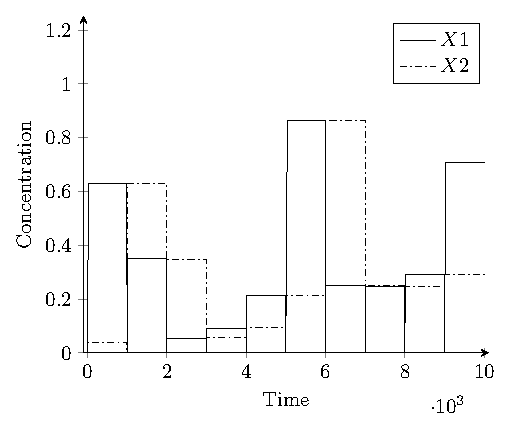
\includegraphics[width=9cm]{ac_3502_as_1957_t_10000_x1_x2}
		\caption{Outputs}
		\label{fig:delay2X1}
	\end{subfigure}
	\caption[Two Stage Backwards Propagating Delay Line I/O]{Two stage backwards propagation delay line showing inputs and outputs. Data arrives as input (\ref{fig:delay2X}) and is available on outputs (\ref{fig:delay2X1}) with $X1$ being the current and $X2$ being the previous $X$.}
	\label{fig:delay2all_A}
\end{figure}

\begin{figure}[ht]
    \centering
	\begin{subfigure}[b]{0.9\textwidth}
	    \centering
		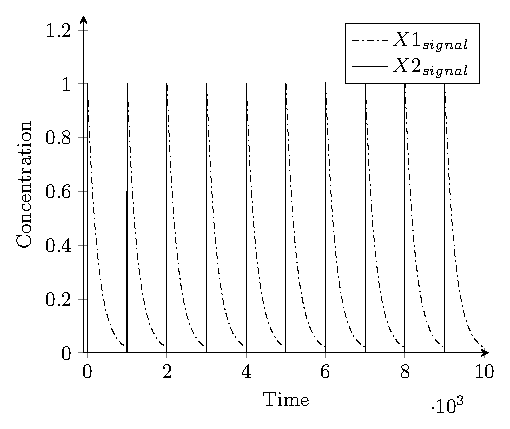
\includegraphics[width=9cm]{ac_3502_as_1957_t_10000_x1signal_x2signal}
		\caption{Copy Signals}
		\label{fig:delay2X2Signal}
		\vspace{15mm}
	\end{subfigure}
	\\
	\begin{subfigure}[b]{0.9\textwidth}
	    \centering
		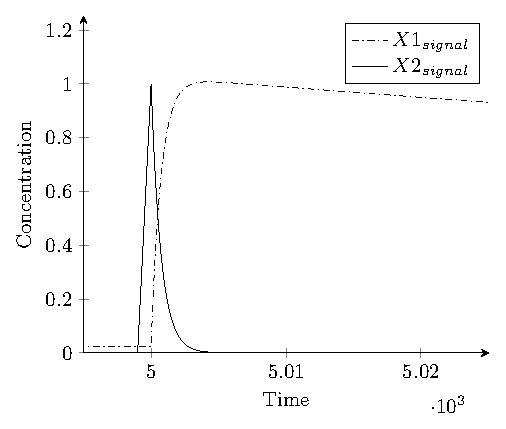
\includegraphics[width=9cm]{ac_3502_as_1957_t_10000_x1signal_x2signal_zoomed}
		\caption{Copy Signals (Zoomed on Figure~\ref{fig:delay2X2Signal})}
		\label{fig:delay2X2SignalZoomed}
	\end{subfigure}
	\caption[Two Stage Backwards Propagating Delay Line Signaling]{Two stage backwards propagation delay line showing copy signaling. The copy is started by $X1_{signal}$ and $X2_{signal}$ (\ref{fig:delay2X2Signal}). Figure~\ref{fig:delay2X2SignalZoomed} shows the signals controlling propagation zoomed in from Figure~\ref{fig:delay2X2Signal}.}
	\label{fig:delay2all_B}
\end{figure}

\subsection{Inherit Single Instruction, Multiple Data}
With the nature of chemistry, one of the advantages of our unconventional delay line implementation is the ability to perform single instruction, multiple data~\cite{Flynn1972-sd} operations. The main factor is finding a unique set of species to hold each delay line that will not react with surrounding buffers to allow such parallel operations. Figure~\ref{fig:simd} shows an example of a two-stage set of backwards propagation and \glspl{mdl} that are producing a vector of three values for the current and previous cycles.

\begin{figure}[ht]
	\centering
		\begin{tikzpicture}
		[inp/.style={rectangle,draw=black!75,fill=Accent-4-1,thick},
		 delay/.style={rectangle,draw=black!100,fill=Accent-4-2,thick,align=left},
		 res/.style={rectangle,draw=white!0,fill=white!20,thick,align=left}]

		\node[inp] 		(input)								{$X2_{signal}$};
		\node[delay]	(delay1)	[right=of input]		{2-stage BPDL};
		\node[delay]	(delay2)	[below=of delay1]		{2-stage BPDL};
		\node[delay]	(delay3)	[below=of delay2]		{2-stage MCDL};

		\node[res]		(res1)		[right=of delay1]		{$X[0][0]$ \\ $X[-1][0]$};
		\node[res]		(res2)		[right=of delay2]		{$X[0][1]$ \\ $X[-1][1]$};
		\node[res]		(res3)		[right=of delay3]		{$X[0][2]$ \\ $X[-1][2]$};

		\node[inner sep = 0, minimum size = 0] (k) at ($(input.east)!0.5!(delay1.west)$) {};


		\draw[->,thick] (input.east) -- (k) |- (delay1.west);
		\draw[->,thick] (input.east) -- (k) |- (delay2.west);
		\draw[->,thick] (input.east) -- (k) |- (delay3.west);

		\draw[->,thick] (delay1.east) -- (res1.west);
		\draw[->,thick] (delay2.east) -- (res2.west);
		\draw[->,thick] (delay3.east) -- (res3.west);
	\end{tikzpicture}
	\caption[Single Instruction, Multiple Data Representation with Delay Line]{Time delay design \gls{simd} representation showing simultaneous output of previous ($X[-1][n]$) and current ($X[0][n]$) $X$ for parallel data processing. The signaling can be used with multiple instances of a delay line, both for the manual copy and the back propagation type.}
	\label{fig:simd}
\end{figure}

\subsection{More than Two Stages}
Extending the buffer for more than two stages is straightforward. For each stage we add one output species ($Xm$), transition species ($XmC$), and catalyst species ($Xm_{signal}$). This allows the system to flexibly provide a buffer of desired length. As an example, Figure~\ref{fig:delayelement3} shows a \gls{bpl} with three stages. The total number of species required in the system grows at a rate of $3m+1$, where $m$ is equal to the number of stages in the system. One trade-off to note is that as the number of stages in the system increases, so does the period of time to cascade values through the delay line. Ideally, each reaction runs to full completion prior to $Xm_{signal}$ propagating backwards to begin the next conversion.

\begin{figure}[ht]
	\centering
	\begin{tikzpicture}
		[t1/.style={circle,draw=black!100,fill=Accent-4-1,thick},
		 tsig/.style={circle,draw=black!100,fill=Accent-4-1,thick},
		 t2/.style={circle,draw=black!100,fill=Accent-4-2,thick},
		 t3/.style={circle,draw=black!100,fill=Accent-4-3},
		 lmb/.style={circle,draw=white!100,fill=white!50}]

		\node[t1]	(xinj)		{$X$};
		\node[t2]	(x1)		[below right=of xinj]	{$X1$};
		\node[t3]	(x1c)		[below left=of xinj]	{$X1C$};
		\node[t2]	(x2)		[below right=of x1c]	{$X2$};
		\node[t3]	(x2c)		[below left=of x1c]		{$X2C$};
		\node[tsig]	(x2sig)		[left=of x1c]			{$X2_{signal}$};
		\node[tsig] (x1sig)     [left=of xinj]			{$X1_{signal}$};			
		\node[tsig]	(x3sig)		[left=of x2c]			{$X3_{signal}$};
		\node[t3]	(x3c)		[below left=of x2c]		{$X3C$};
		\node[t2]	(x3)		[below right=of x2c]	{$X3$};
		\node[lmb]  (lamb)		[above=of x1sig]		{$\lambda$};

		\node[scale=0.2]	(syr1)		[above right=-0.1cm of xinj]	{\syringePDFImage};
		\node[scale=0.2,rotate=90]	(syr2)		[above left=0.1cm of x3sig]	{\syringePDFImage};

		\draw[->,thick] (xinj.south) -- ($(x1c.north)!0.5!(x1.north)$) to[out=-90,in=0] (x1c.east);
		\draw[->,thick] (xinj.south) -- ($(x1c.north)!0.5!(x1.north)$) to[out=-90,in=180] (x1.west);

		\draw[->,thick] (x1c.south) -- ($(x2c.north)!0.5!(x2.north)$) to[out=-90,in=0] (x2c.east);
		\draw[->,thick] (x1c.south) -- ($(x2c.north)!0.5!(x2.north)$) to[out=-90,in=180] (x2.west);

		\draw[->,thick] (x2c.south) -- ($(x3c.north)!0.5!(x3.north)$) to[out=-90,in=180] (x3.west);
		\draw[->,thick] (x2c.south) -- ($(x3c.north)!0.5!(x3.north)$) to[out=-90,in=0] (x3c.east);

		\draw[->,dashed,thick] (x1sig.south east) -- ($(x1c.north)!0.5!(x1.north)$);
		\draw[->,dashed,thick] (x2sig.south east) -- ($(x2c.north)!0.5!(x2.north)$);
		\draw[->,dashed,thick] (x3sig.south east) -- ($(x3c.north)!0.5!(x3.north)$);

		\draw[->,thick] (x2sig.north) to[out=90,in=180] (x1sig.west);
		\draw[->,thick] (x3sig.north) to[out=90,in=180] (x2sig.west);

		\draw[->,thick] (x1sig.north) to[out=90,in=270] (lamb.south);
	\end{tikzpicture}
	\caption[Three Stage Backwards Propagating Delay Line]{\Gls{bpl} with three stages. The syringe is used to indicate an injection of the input $X$ and the signal $X3_{signal}$. Species $X1$, $X2$, and $X3$ represent the output species from the delay line. Lambda ($\lambda$) shows decay of backwards propagation signal.}
	\label{fig:delayelement3}
\end{figure}

The reaction set of the delay line also scales in a straightforward fashion. Each intermediate delay stage has a reaction similar to reaction~\ref{eq:Xreac} and the final delay stage (the $m^{th}$ delay) has a reaction similar to reaction~\ref{eq:X1Creac}. This remains true for extending both the manual and backwards propagating delay line. Extension of the catalysts depends on the implementation. For the \gls{mdl}, simply adding the species and a subsequent input is required. Extending the backward propagating delay line has the advantage that it does not increase the number of injections, but it still increases the overall number of species.

\section{Results}
\label{sec:dl_results}
We will highlight the results for the two stage buffer and its extension beyond two stages. We employed Genetic Algorithms (GAs)~\cite{Mitchell1998-tw} to optimize the rate constants (mapped to chromosomes) of the backwards propagation model. We only used the algorithm to optimize the backwards propagation model since the manual copy was straightforward to optimize by hand. The GA used an elite selection of the top 20 chromosomes from the population of 100, which undergo cross-over and mutation to form the next generation. The goal (fitness function) of this evolutionary algorithm was to minimize the error of the delay line.

We defined error as the difference between the actual input value ($X$) and the value occurring at $X1$ on this cycle and then $X2$ on the next cycle. We performed this test 50 time steps after $X$ is injected into the delay line. Equation~\ref{eq:errorequation} shows the calculation of this error where $X[n]$ represents the current value of $X$ and $X[n-1]$ represents the value of $X$ on the previous input cycle. Adding both differences for the two stage delay line provided the overall error.

\begin{equation}
error = |X_1 - X[n]| + |X_2 - X[n-1]| \label{eq:errorequation}
\end{equation}

The genetic algorithm performed perturbation mutation that changed each chromosome's element with 30\% chance by $\pm$30\% using a uniform distribution. We ran the GA for 100 generations to produce the results for the two stage delay line. The algorithm was configured to target a transition of the input species, $X$, to the current time species, $X1$, as fast as possible, and convert the intermediate species, $X1C$ to the previous time species, $X2$, as fast as possible while minimizing the amount of leakage between the phases of the design.

\subsection{Two Stages}
Table~\ref{tab:rateconstantsMan} shows the rate constants for the manual propagation delay line reactions. Rates for the conversion of input species, $X$, down the chain is the same rate with the presence of $X1_{signal}$ and $X2_{signal}$ both increasing the rate by the same amount because the forward copy reactions should be as fast as possible. Figures~\ref{fig:delay2allMan_A} and \ref{fig:delay2allMan_B} shows the plots using these rate constants in a two stage system, which can be replicated for a manual copy system of any size.

\begin{table}[ht]
    \caption[Two Stage Manual Copy Delay Line Rate Constants]{Rate constants of two stage \gls{mdl} found by GA.}
    \label{tab:rateconstantsMan}
    \centering
    \begin{tabular}{llll}
	    Reaction                                 & Forward Rate & $K_m$          \\ \hline
	    $X \xrightarrow{X1_{signal}} X1 + X1C$   & 0.0757       & 2.0000         \\
	    $X1C \xrightarrow{X2_{signal}} X2 + X2C$ & 0.0757       & 2.0000         \\
		$X2_{signal} \rightarrow \lambda$        & 0.5643       & (None)         \\
	    $X1_{signal} \rightarrow \lambda$        & 0.5643       & (None)         \\
    \end{tabular}
\end{table}

For a different size, the back propagation delay line has different rate constants. In addition, the rate constants were not grouped like the manual propagation delay line because it would drastically decrease the performance. Looking at the constants in Table~\ref{tab:rateconstants}, the reaction for species $X1C$ to $X2$ is the fastest. This is directly due to the rapid rate that $X2_{signal}$ is reacting to $X1_{signal}$. Effectively, to meet the first requirement of getting $X$ into $X1$ as fast as possible, the lower level transition of species (Reaction~\ref{eq:X1Creac}) must complete before. Figures~\ref{fig:delay2all_A} and \ref{fig:delay2all_B} shows the output of a two stage \gls{bpl} with the rate constants in Table~\ref{tab:rateconstants}.

\begin{table}
    \caption[Two Stage Backwards Propagating Delay Line Rate Constants]{Rate constants of two stage \gls{bpl} found by GA.}
    \label{tab:rateconstants}
    \centering
    \begin{tabular}{llll}
	    Reaction                                 & Forward Rate & $K_m$          \\ \hline
	    $X \xrightarrow{X1_{signal}} X1 + X1C$   & 0.0020       & 0.0225         \\
	    $X1C \xrightarrow{X2_{signal}} X2 + X2C$ & 0.0706       & 2.0000         \\
	    $X2_{signal} \rightarrow X1_{signal}$    & 1.3648       & (None)         \\
	    $X1_{signal} \rightarrow \lambda$        & 0.0039       & (None)         \\
    \end{tabular}
\end{table}

To compare the accumulated error of the two delay lines we used symmetric mean absolute percentage error (SAMP) defined as
\begin{equation}
SAMP = 100 * \langle \frac{|y-\hat{y}|}{y+\hat{y}} \rangle,
\end{equation}
where $\langle.\rangle$ is the mean of a set of multiple values, $y$ is the actual value, and $\hat{y}$ is the expected value. We calculated an average SAMP per stage (unit size) by dividing cumulative SAMP with $m$. More specifically, using $n$ to represent a discrete time series sample and $m$ to represent the number of stages:
\begin{equation}
SAMP = \frac{100}{m} * \sum \limits_{k=1}^{m} \langle \frac{|Xk-X[n-(k-1)]|}{Xk+X[n-(k-1)]} \rangle.
\end{equation}
For instance, SAMP for two stages ($m=2$) is given by
\begin{equation}
SAMP = \frac{100}{2} * \langle \frac{|X1-X[n]|}{X1+X[n]} + \frac{|X2-X[n-1]|}{X2+X[n-1]} \rangle \label{eq:sampn2}.
\end{equation}

We evaluated performance (error) over 10,000 runs, each repeating the sequence of actions defined in Table~\ref{tab:as2Man} and Table~\ref{tab:as2} for 200 iterations (200,000 time steps). Figure~\ref{fig:fiveStageAbsDiff} shows the results for a delay line of size two as well as for larger sizes (discussed in next section). The difference in values from expected values for the two stage delay line are quite small. This shows that for a two stage delay line, both types operate well. One thing to note is that the backwards delay line has a larger initial error which can accumulate over time.

\subsection{Over Two Stages}
\label{sec:dl_paper_over_two_stages}
In this section, we will examine the use of a delay line with five stages. Five stages was selected and executed for both the manual copy and back propagating delay line. Figure~\ref{fig:fiveStageAbsDiff} shows the final error when evaluated for 10,000 runs for 200 iterations each (same as for $m=2$ in previous section). The maximum error over the entire evaluation is shown in Table~\ref{tab:maxSAMP}. There are a few observations to note on this plot. The error on a backwards propagation delay line ($B$) increases as the number of stages in the delay line increases. For a smaller delay line, this error would generally be negligible, but for larger sizes this could be a concern. The manual copy has a significantly smaller error as shown in Figure~\ref{fig:fiveStageAbsDiff}.

\begin{figure}[ht]
	\centering
	\begin{tikzpicture}
		\begin{axis}[
		xlabel={Step},
		ylabel={SAMP},
		xticklabel style={/pgf/number format/fixed},
		enlargelimits=true,
		cycle multi list={Mark-Dark2-8},
		legend style={
			legend pos=outer north east,
			legend columns=1,
		},
		ymode=log,
		axis x line=bottom,
		axis y line=left,
		width=13cm,
		height=7.313cm,
		mark repeat=20,
		]
			\addplot table [x=Step, y=manual2, col sep=comma] {data/performance_back_manual.csv};
			\addplot table [x=Step, y=manual5, col sep=comma] {data/performance_back_manual.csv};
			\addplot table [x=Step, y=manual10, col sep=comma] {data/performance_back_manual.csv};

			\addplot table [x=Step, y=back2, col sep=comma] {data/performance_back_manual.csv};
			\addplot table [x=Step, y=back3, col sep=comma] {data/performance_back_manual.csv};
			\addplot table [x=Step, y=back4, col sep=comma] {data/performance_back_manual.csv};
			\addplot table [x=Step, y=back5, col sep=comma] {data/performance_back_manual.csv};
			\legend{M2, M5, M10, B2, B3, B4, B5}
        \end{axis}
	\end{tikzpicture}
	\caption[Error for Both Delay Lines]{SAMP calculated for delay lines. M$m$ and B$m$ are the $m^{th}$ stage of manual copying and back propagation delay line.}
	\label{fig:fiveStageAbsDiff}
\end{figure}

\begin{table}[ht]
	\centering
	\caption[Error for Both Delay Lines]{Maximum and average SAMP obtained through performance runs of 200 iterations and varying configurations of stages and manual copy and backwards propagation. Maximum and average excludes the initial values where the delay line is filling (first $m$ points with low SAMP).}
	\label{tab:maxSAMP}
	\begin{tabular}{llllll}
	Backwards DL & Max     & Average & Manual DL & Max      & Average  \\ \hline
	B5           & 14.35\% & 14.09\% & M10       & 0.0059\% & 0.0016\% \\
	B4           & 11.66\% & 11.25\% & M5        & 0.0049\% & 0.0024\% \\
	B3           & 5.26\%  & 4.84\%  & M2        & 0.0033\% & 0.0008\% \\
	B2           & 2.28\%  & 1.97\%  & ~         & ~        & ~        \\
	\end{tabular}
\end{table}

As for the backwards propagating delay line, the error starts to accumulate to a noticeable value rapidly. Even by phase three, the delay line is starting to produce error that is in excess of the \gls{mdl} with ten stages. Looking back to Figure~\ref{fig:delay2X2SignalZoomed} there is a period of time where both $X1_{signal}$ and $X2_{signal}$ overlap which can explain how error that starts quite small in stage one of the delay system accumulates to a large value by the time it reaches the later stages of the buffer. Depending on the desired properties of the delay line, this is worth considering for the application.

\subsection{Time Series Perceptron Integration}
To demonstrate the capabilities of the delay line to fit into other designs, we integrated it with a chemical perceptron called a threshold asymmetric signal perceptron introduced by Banda~\cite{Banda2014-bp}. This perceptron learns through reinforcements and is inspired by biological neurons. Integration with the delay line and the perceptron shows how the delay line can easily fit with other systems to act as an input stream without any design modifications. Previously, the perceptron received both values simultaneously as two inputs. Now, we are showing that, without change to the perceptron or delay line, the two integrate together and function well. Figure~\ref{fig:perceptintegrate} shows an example of this integration.

\begin{figure}[ht]
	\centering
		\begin{tikzpicture}
			[t1/.style={circle,draw=black!75,fill=Accent-4-1,thick},
			 t2/.style={circle,draw=black!50,fill=Accent-4-2,thick},
			 t3/.style={circle,draw=black!50,fill=Accent-4-3},
			 t4/.style={circle,draw=black!50,fill=Accent-4-4},
			 lmb/.style={circle,draw=white!100,fill=white!50}]

			\node[t1]	(xinj)								{$X$};
			\node[t2]	(x1)		[below right=of xinj]	{$X1$};
			\node[t3]	(x1c)		[below left=of xinj]	{$X1C$};
			\node[t2]	(x2)		[below=of x1c]			{$X2$};
			\node[t1]	(x2sig)		[left=of x1c]			{$X2_{signal}$};
			\node[t1]   (x1sig)     [left=of xinj]			{$X1_{signal}$};	
			\node[t4]	(percep)	[right=of x2]			{$Perceptron$};
			\node[lmb]  (lamb)		[above=of x1sig]		{$\lambda$};

			\node[scale=0.2]	(syr1)		[above right=-0.1cm of xinj]	{\syringePDFImage};
			\node[scale=0.2,rotate=90]	(syr2)		[above left=0.1cm of x2sig]	{\syringePDFImage};

			\draw[->,thick] (xinj.south) -- ($(x1c.north)!0.5!(x1.north)$) to[out=-90,in=0] (x1c.east);
			\draw[->,thick] (xinj.south) -- ($(x1c.north)!0.5!(x1.north)$) to[out=-90,in=180] (x1.west);

			\draw[->,thick] (x1c.south) -- (x2.north);

			\draw[->,dashed,thick] (x1sig.south east) -- ($(x1c.north)!0.5!(x1.north)$);
			\draw[->,dashed,thick] (x2sig.south east) -- ($(x1c.south)!0.5!(x2.north)$);

			\draw[->,dotted,thick] (x2.east)	to[out=0,in=180]	(percep.west);
			\draw[->,dotted,thick] (x1.south)	to[out=270,in=90]	(percep.north);

			\draw[->,thick] (x2sig.north) to[out=90,in=180] (x1sig.west);
			\draw[->,thick] (x1sig.north) to[out=90,in=270] (lamb.south);

		\end{tikzpicture}
	\caption[Perceptron Integration with Backwards Propagating Delay Line]{Perceptron integration with backwards propagating delay line of two stages. The delay line outputs ($X1$ and $X2$) are fed to the perceptron without modification of the delay line.}
	\label{fig:perceptintegrate}
\end{figure}

We trained the perceptron using reinforcement learning on 14 linearly separable binary function. Figure~\ref{fig:perceptLearning} shows the results of this learning. The binary time series perceptron learns 11 of the 14 functions with an accuracy of greater than 85\%. Figure~\ref{fig:ORPerceptResults} shows the buffer and perceptron accurately producing the output for OR.

\begin{figure}[ht]
	\centering
	\begin{subfigure}[b]{0.9\textwidth}
	    \centering
    	\begin{tikzpicture}
    		\begin{axis}[
    		xlabel={Step},
    		ylabel={Success Rate},
    		xticklabel style={/pgf/number format/fixed},
    		cycle multi list={Mark-Dark2-8},
    		legend style={
    			legend pos=south east,
    			legend columns=4,
    		},
    		enlarge x limits = false,
    		width=13cm,
    		height=7.313cm,
    		mark repeat=20,
    		]
    			\addplot table [x=Step, y=CONST1, col sep=comma] {data/performance_2483-2498.csv};
    			\addplot table [x=Step, y=CONST0, col sep=comma] {data/performance_2483-2498.csv};
    			\addplot table [x=Step, y=OR, col sep=comma] {data/performance_2483-2498.csv};
    			\addplot table [x=Step, y=CIMPL, col sep=comma] {data/performance_2483-2498.csv};
    			\addplot table [x=Step, y=PROJX1, col sep=comma] {data/performance_2483-2498.csv};
    			\addplot table [x=Step, y=IMPL, col sep=comma] {data/performance_2483-2498.csv};
    			\addplot table [x=Step, y=PROJX2, col sep=comma] {data/performance_2483-2498.csv};
    			\legend{CONST1,CONST0,OR,CIMPL,PROJX1,IMPL,PROJX2}
            \end{axis}
    	\end{tikzpicture}
    \end{subfigure}
    \\
    \begin{subfigure}[b]{0.9\textwidth}
        \centering
		\begin{tikzpicture}
		\begin{axis}[
		xlabel={Step},
		ylabel={Success Rate},
		xticklabel style={/pgf/number format/fixed},
		cycle multi list={Mark-Dark2-8},
		legend style={
			legend pos=south east,
			legend columns=4,
		},
		enlarge x limits = false,
		width=13cm,
		height=7.313cm,
		mark repeat=20,
		]
			\addplot table [x=Step, y=AND, col sep=comma] {data/performance_2483-2498.csv};
			\addplot table [x=Step, y=NAND, col sep=comma] {data/performance_2483-2498.csv};
			\addplot table [x=Step, y=NOTX2, col sep=comma] {data/performance_2483-2498.csv};
			\addplot table [x=Step, y=NIMPL, col sep=comma] {data/performance_2483-2498.csv};
			\addplot table [x=Step, y=NOTX1, col sep=comma] {data/performance_2483-2498.csv};
			\addplot table [x=Step, y=NCIMPL, col sep=comma] {data/performance_2483-2498.csv};
			\addplot table [x=Step, y=NOR, col sep=comma] {data/performance_2483-2498.csv};
			\legend{AND,NAND,NOTX2,NIMPL,NOTX1,NCIMPL,NOR}
        \end{axis}
	\end{tikzpicture}
\end{subfigure}
	
	\caption[Success Rate with Delay Line and Perceptron Integration]{Success rate of binary time series chemical perceptron. The perceptron learns 11 of the 14 linearly separable functions with an accuracy of greater than 85\%.}
	\label{fig:perceptLearning}
	
\end{figure}

\begin{figure}[p]
	\centering
	\begin{subfigure}[b]{0.9\textwidth}
	    \centering
		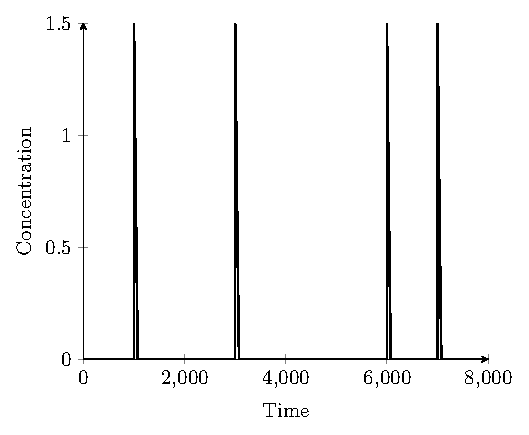
\includegraphics[width=9cm]{or_input}
		\caption{Input Stream}
		\label{fig:ORinput}
		\vspace{15mm}
	\end{subfigure}
	\\
	\begin{subfigure}[b]{0.9\textwidth}
	    \centering
		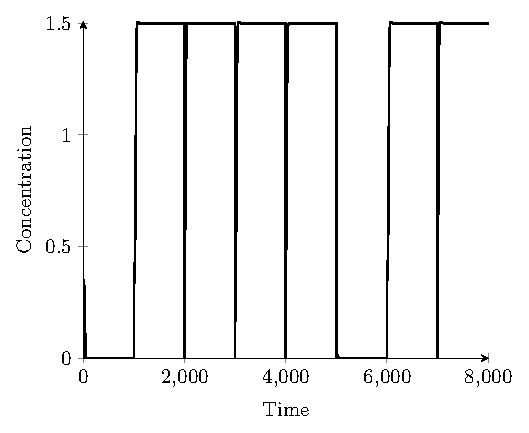
\includegraphics[width=9cm]{or_output}
		\caption{Output Stream}
		\label{fig:OROutput}
	\end{subfigure}
	\caption[Concentration Traces for Perceptron/Delay Line Learning Logic OR]{Example concentration traces of binary time series chemical perceptron that successfully learns OR function. Left shows input stream 0,1,0,1,0,0,1,1. Right shows correct output stream of 0,1,1,1,1,0,1,1. Two zeros on the input stream at 4,000 and 5,000 successfully produce zero at time 5,000 on output stream.}
	\label{fig:ORPerceptResults}
\end{figure}

NAND, IMPL, and NOTX1 are all heavily dependent on the last input to resolve in the time delay line, $X1$. The input species $X1$ is not provided to the system until typically 50 time steps later than value $X2$. The original model of the perceptron was optimized for instantaneous and simultaneous injection of both inputs. Because input $X1$ is not ready, the performance is lower because that input plays a larger role on the correct performance for these logic functions. This makes the system capable of obtaining an average success rate of approximately 90\% compared to the perceptron's 99\% success rate~\cite{Banda2014-bp}.

\section{Deoxyribozyme Cascading Implementation}
\label{sec:deoxy}
Now, we would like to present how such a delay line could be realized in a system employing deoxyribozyme catalysis~\cite{Stojanovic2003-eg}~\cite{Stojanovic2000-qx}~\cite{Liu2009-jz}. Figure~\ref{fig:deoxy1} shows an example of a two stage manual delay line with the signals being the deoxyribozymes $X1_{signal}$ and $X2_{signal}$ which cleave the substrate $X$ at the embedded ribonucleotide. This produces $X1$ ready for the next system to consume. Subsequently, $X1C$ embedded with another ribonucleotide is able to get cleaved by deoxyribozyme $X2_{signal}$ to form the next input to the system, $X2$.

\begin{figure}[ht]
	\centering
	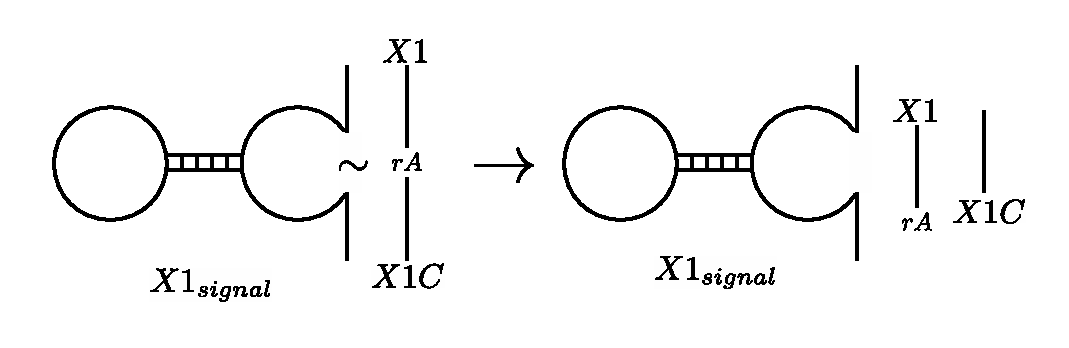
\includegraphics[width=12cm]{cleavage}
	\caption[Example of Deoxyribozyme Implementation]{Deoxyribozyme cascading example. Deoxyribozyme $X1_{signal}$ cleaves $X$ at embedded ribonucleotide ($rA$) to form $X1$ and $X1C$. A similar process occurs on $X1C$ to produce $X2$ and $X2C$.}
	\label{fig:deoxy1}
\end{figure}

\section{Discussion}
We have presented a novel implementation of a delay line as a chemical reaction network capable of storing past concentrations. By arranging our delay lines in a SIMD-like layout, we could delay multiple segments of data simultaneously with a shared control signal for either model of delay line. We have introduced two types of a chemical delay line: manual copy delay line and backwards propagation delay line. A manual copy delay line can precisely carry values in a delayed state, but requires more intervention from the user (growing at a rate of $m$) to propagate values through the system. The second model, backwards propagating delay line, automatically moves values through the system with a single signaling injection with reasonable accuracy.

The integration of the backwards propagating delay line with the threshold asymmetric signal perceptron resulted in the first chemical model capable of learning binary time series. Also, this example is a proof-of-concept that our delay line is a modular block ready for use in other systems. For systems requiring a smaller window of past values, either model of the delay line gives sufficient accuracy for data storage. The manual copy delay line shows potential for longer chains with the amount of calculated SAMP passed between phases remaining below 0.01\% for a delay line of 10 stages. The backwards propagating delay line provides a much simpler user interface at the sacrifice of accuracy. A backwards propagation of five stages keeps the calculated SAMP below 15\%. Systems requiring a large number of delays will have to weigh accuracy and simplicity to make a selection for a particular implementation.

The \gls{bpl} and \gls{mdl} tied with a \gls{asp} demonstrate how these two systems can modularly connect to other elements in a \gls{crn} to form a memory. Now that there are the building blocks to provide data storage in a \gls{crn}, we discuss the work to find the optimal size of memory and layout of \gls{ann} to solve the ant trail task when paired with a delay line.


